\textbf{Model uczony na stałej krzywiźnie wierzechołków}

% \begin{figure}[ht]
% 	\centering
% 	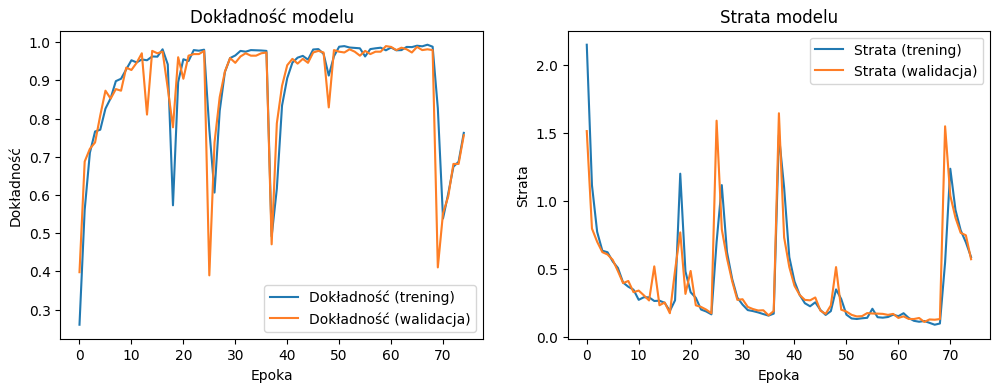
\includegraphics[height=5.5cm]{resources/tests/images/v2/base4_img.png}
% 	\caption{Wyniki testów dla modelu podstawowego ze stałą krzywizną wierzechołków, liczba wierzchołków = 4}
% 	\label{Fig:tests-base-1}
% \end{figure}
% \FloatBarrier

% \begin{figure}[ht]
% 	\centering
% 	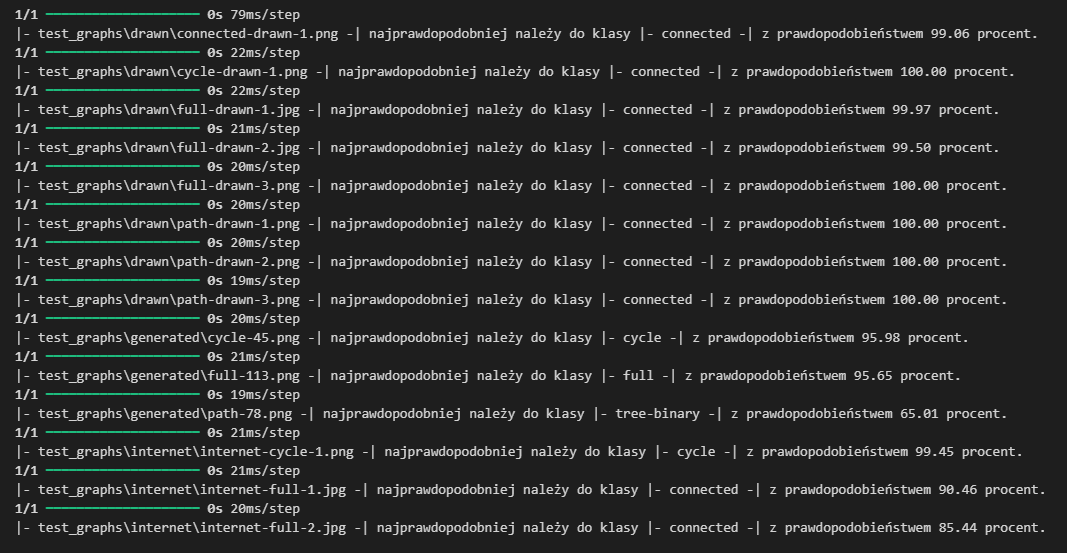
\includegraphics[height=7cm]{resources/tests/images/v2/base4_txt.png}
% 	\caption{Klasyfikacja obrazów zewnętrznych dla modelu podstawowego ze stałą krzywizną wierzechołków, liczba wierzchołków = 4}
% 	\label{Fig:tests-base-2}
% \end{figure}
% \FloatBarrier

% \begin{figure}[ht]
% 	\centering
% 	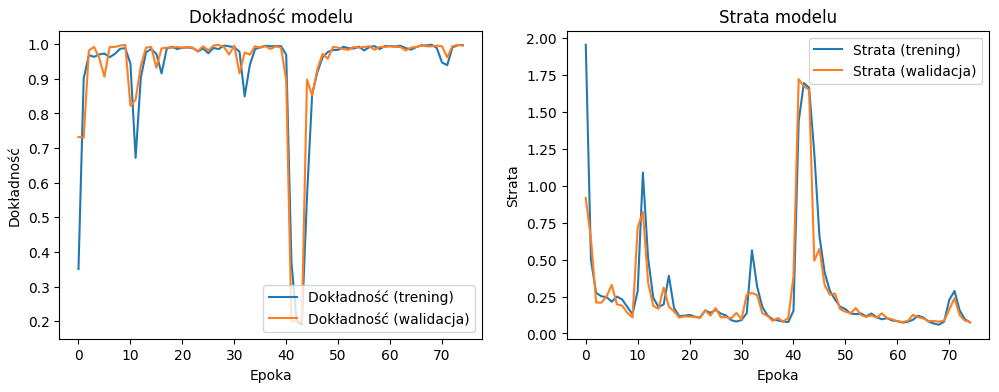
\includegraphics[height=5.5cm]{resources/tests/images/v2/base5_img.png}
% 	\caption{Wyniki testów dla modelu podstawowego ze stałą krzywizną wierzechołków, liczba wierzchołków = 5}
% 	\label{Fig:tests-base-1}
% \end{figure}
% \FloatBarrier

% \begin{figure}[ht]
% 	\centering
% 	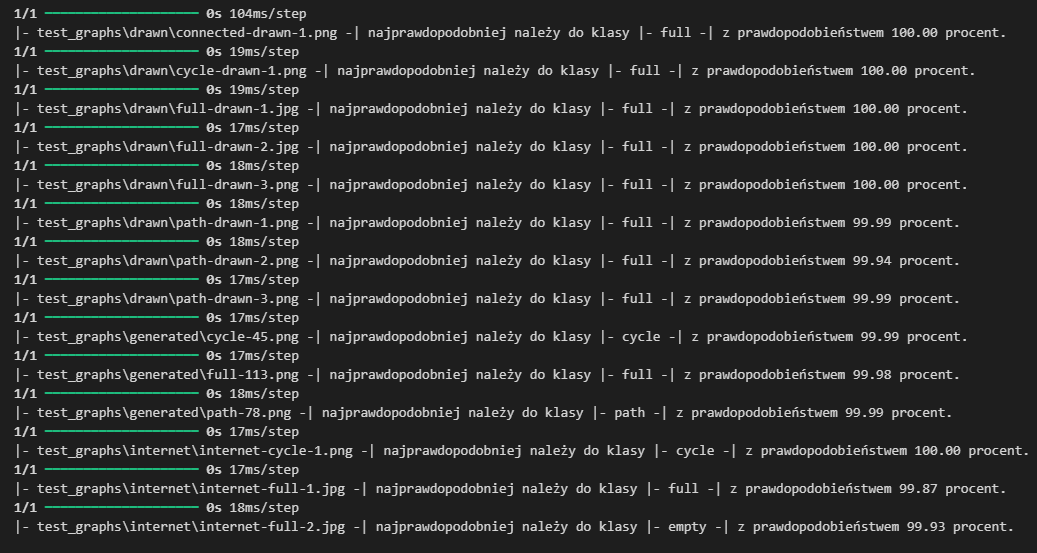
\includegraphics[height=7cm]{resources/tests/images/v2/base5_txt.png}
% 	\caption{Klasyfikacja obrazów zewnętrznych dla modelu podstawowego ze stałą krzywizną wierzechołków, liczba wierzchołków = 5}
% 	\label{Fig:tests-base-2}
% \end{figure}
% \FloatBarrier

% \begin{figure}[ht]
% 	\centering
% 	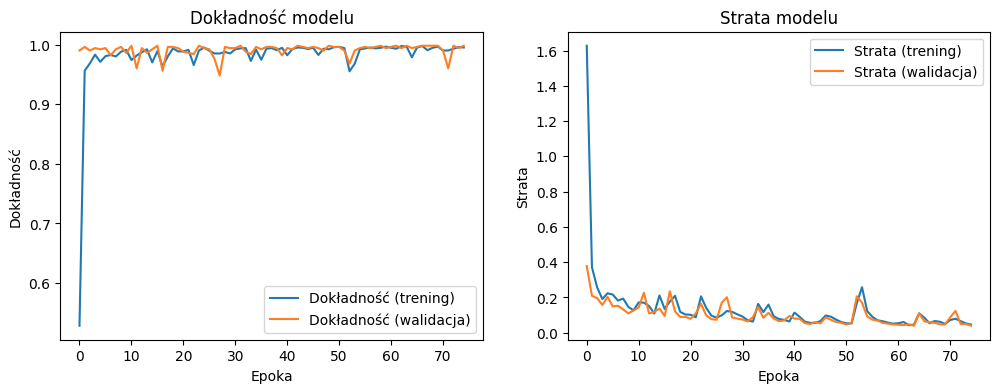
\includegraphics[height=5.5cm]{resources/tests/images/v2/base6_img.png}
% 	\caption{Wyniki testów dla modelu podstawowego ze stałą krzywizną wierzechołków, liczba wierzchołków = 6}
% 	\label{Fig:tests-base-1}
% \end{figure}
% \FloatBarrier

% \begin{figure}[ht]
% 	\centering
% 	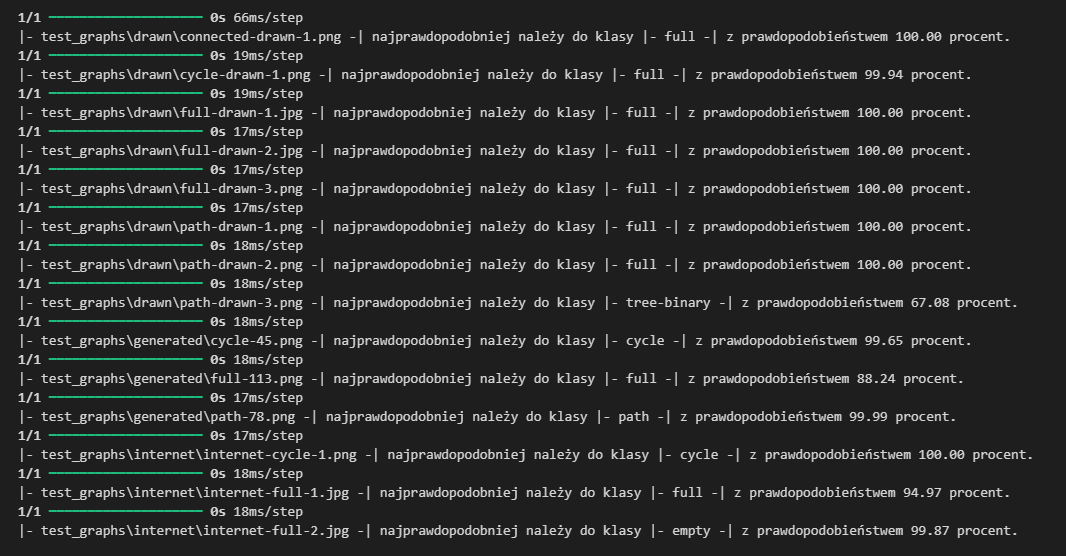
\includegraphics[height=7cm]{resources/tests/images/v2/base6_txt.png}
% 	\caption{Klasyfikacja obrazów zewnętrznych dla modelu podstawowego ze stałą krzywizną wierzechołków, liczba wierzchołków = 6}
% 	\label{Fig:tests-base-2}
% \end{figure}
% \FloatBarrier

% \begin{figure}[ht]
% 	\centering
% 	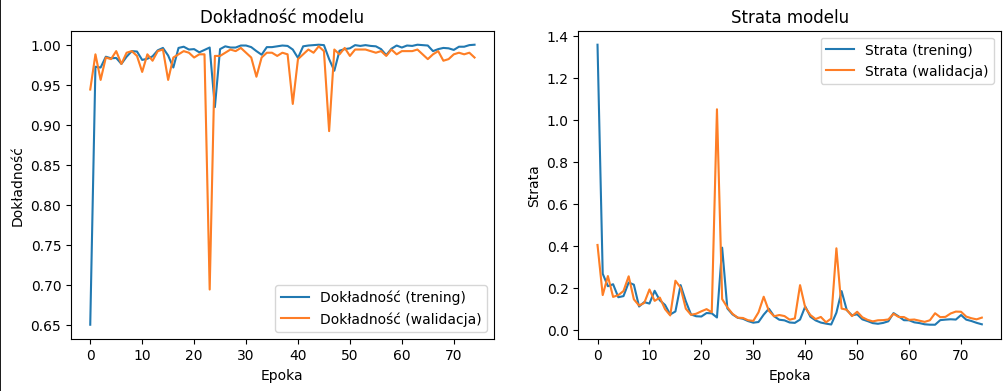
\includegraphics[height=5.5cm]{resources/tests/images/v2/base7_img.png}
% 	\caption{Wyniki testów dla modelu podstawowego ze stałą krzywizną wierzechołków, liczba wierzchołków = 7}
% 	\label{Fig:tests-base-1}
% \end{figure}
% \FloatBarrier

% \begin{figure}[ht]
% 	\centering
% 	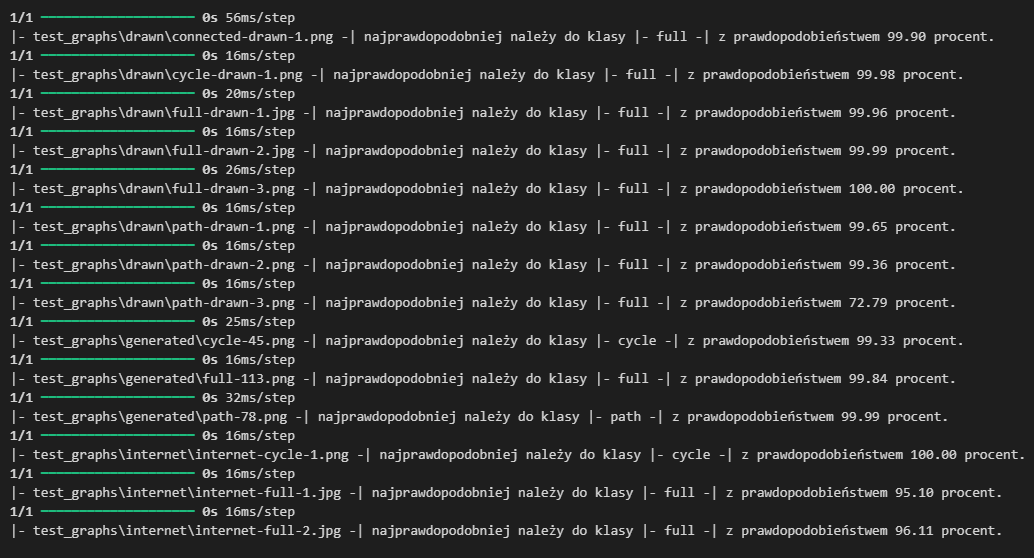
\includegraphics[height=7cm]{resources/tests/images/v2/base7_txt.png}
% 	\caption{Klasyfikacja obrazów zewnętrznych dla modelu podstawowego ze stałą krzywizną wierzechołków, liczba wierzchołków = 7}
% 	\label{Fig:tests-base-2}
% \end{figure}
% \FloatBarrier

\textbf{Model uczony na losowej krzywiźnie wierzechołków}

Dokładność modelu podstawowego, uczonego na grafach z czterema wierzchołkami stopniowo rosnie,
zaczynając od około 40\% i osiągając prawie 90\% pod koniec procesu uczenia.
Może to sugoerować, że model dobrze uczy się na danych treningowych.
Dokładność na danych walidacyjnych jest zbliżona do wcześniej przytoczonej.
Wskazuje to, że model dobrze radzi sobie z generalizacją na nowych danych.

Strata na danych treningowych gwałtownie spada z około 1.75 do około 0.25 w ciągu pierwszych dziesięciu epok,
po czym stabilizuje się.
Wskazuje to na szybkie uczenie się na na danych treningowych.
Strata na danych walidacyjnych jest nieznacznie bardziej zmienna,
z kilkoma wzrostami w późniejszych epokach.
Może to sugerować trudności z generalizacją na nowych danych.

\begin{figure}[ht]
	\centering
	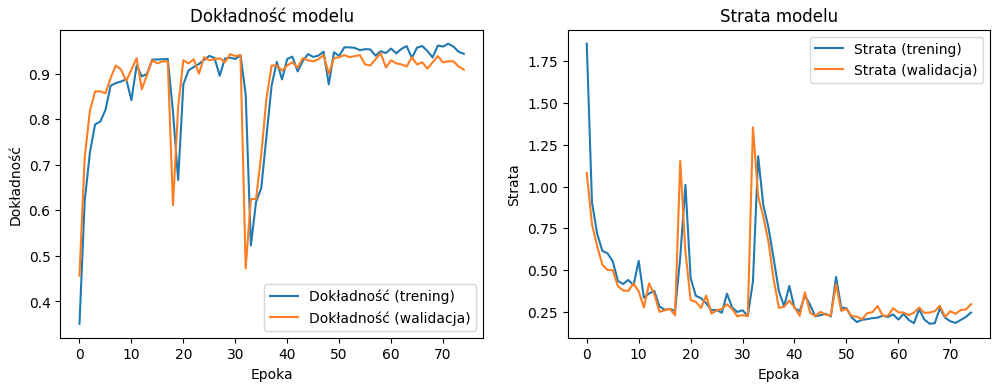
\includegraphics[height=5.5cm]{resources/tests/images/v3/base4_img.png}
	\caption{Wyniki testów dla modelu podstawowego z losową krzywizną wierzechołków, liczba wierzchołków = 4}
	\label{Fig:tests-base-1}
\end{figure}
\FloatBarrier

Ogólnie rzecz biorąc, model wydaje się dobrze uczyć na danych treningowych i generalizować na danych walidacyjnych,
chociaż zmienność straty walidacyjnej może wskazywać na pewne problemy z przeuczeniem.

\begin{figure}[ht]
	\centering
	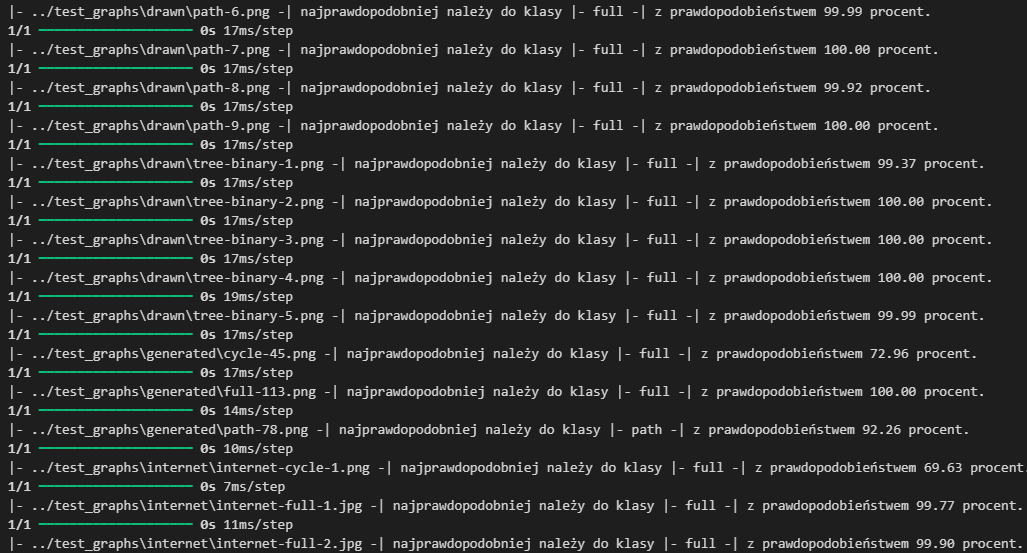
\includegraphics[height=7cm]{resources/tests/images/v3/base4_txt.png}
	\caption{Klasyfikacja obrazów zewnętrznych dla modelu podstawowego z losową krzywizną wierzechołków, liczba wierzchołków = 4}
	\label{Fig:tests-base-2}
\end{figure}
\FloatBarrier

Model przewidział poprawnie 50\% grafów, co nie jest najgorszym wynikiem,
zaważając że jest to najbardziej podstawowa wersja testowanego modelu.

\begin{figure}[ht]
	\centering
	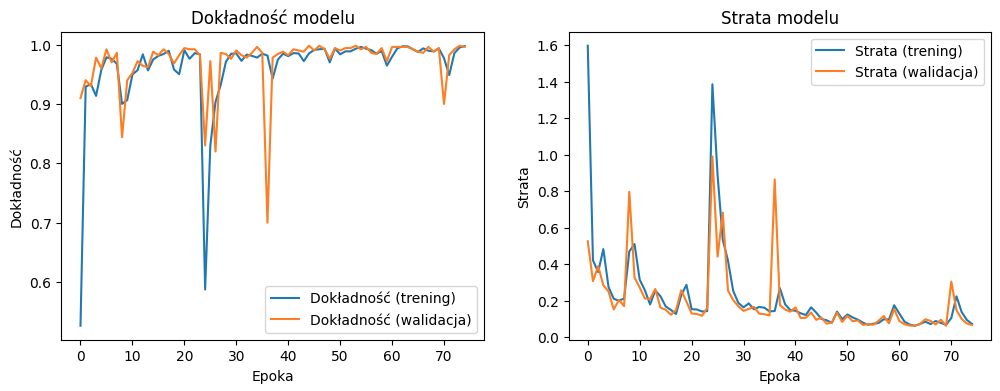
\includegraphics[height=5.5cm]{resources/tests/images/v3/base5_img.png}
	\caption{Wyniki testów dla modelu podstawowego z losową krzywizną wierzechołków, liczba wierzchołków = 5}
	\label{Fig:tests-base-1}
\end{figure}
\FloatBarrier

\begin{figure}[ht]
	\centering
	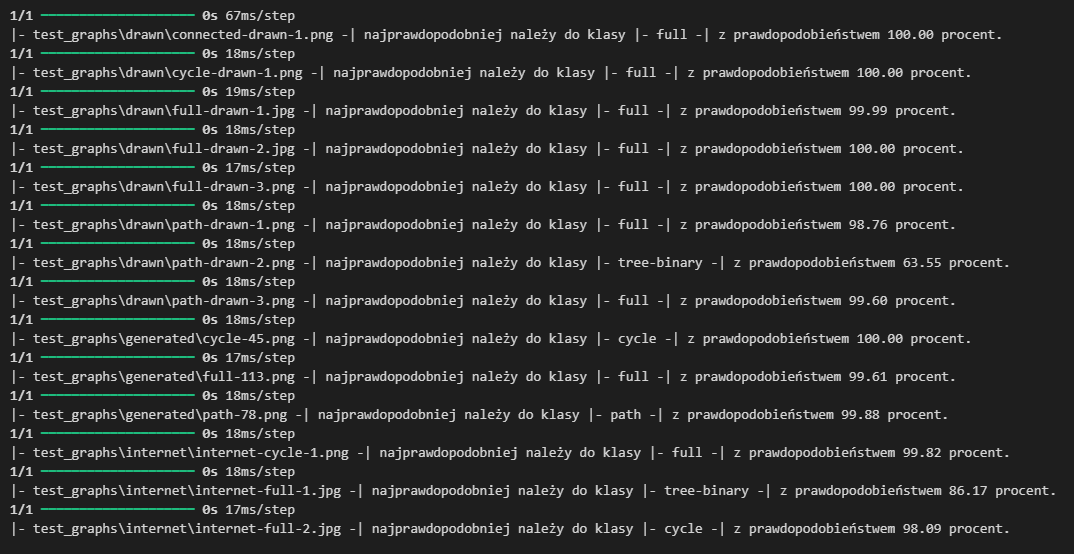
\includegraphics[height=7cm]{resources/tests/images/v3/base5_txt.png}
	\caption{Klasyfikacja obrazów zewnętrznych dla modelu podstawowego z losową krzywizną wierzechołków, liczba wierzchołków = 5}
	\label{Fig:tests-base-2}
\end{figure}
\FloatBarrier

\begin{figure}[ht]
	\centering
	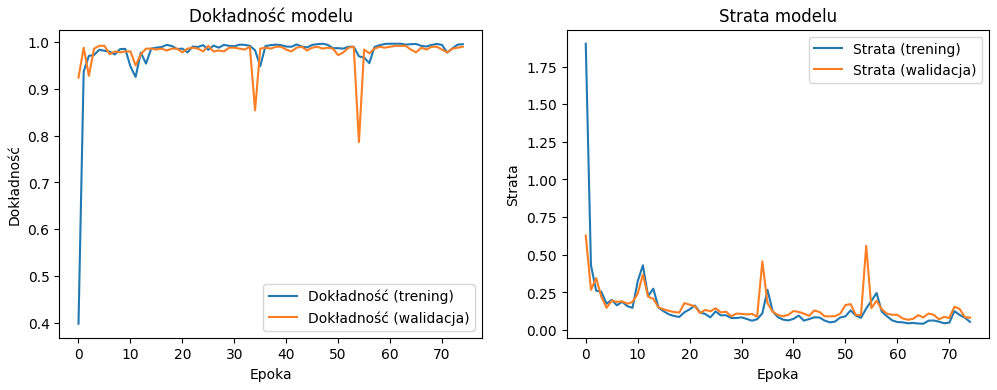
\includegraphics[height=5.5cm]{resources/tests/images/v3/base6_img.png}
	\caption{Wyniki testów dla modelu podstawowego z losową krzywizną wierzechołków, liczba wierzchołków = 6}
	\label{Fig:tests-base-1}
\end{figure}
\FloatBarrier

\begin{figure}[ht]
	\centering
	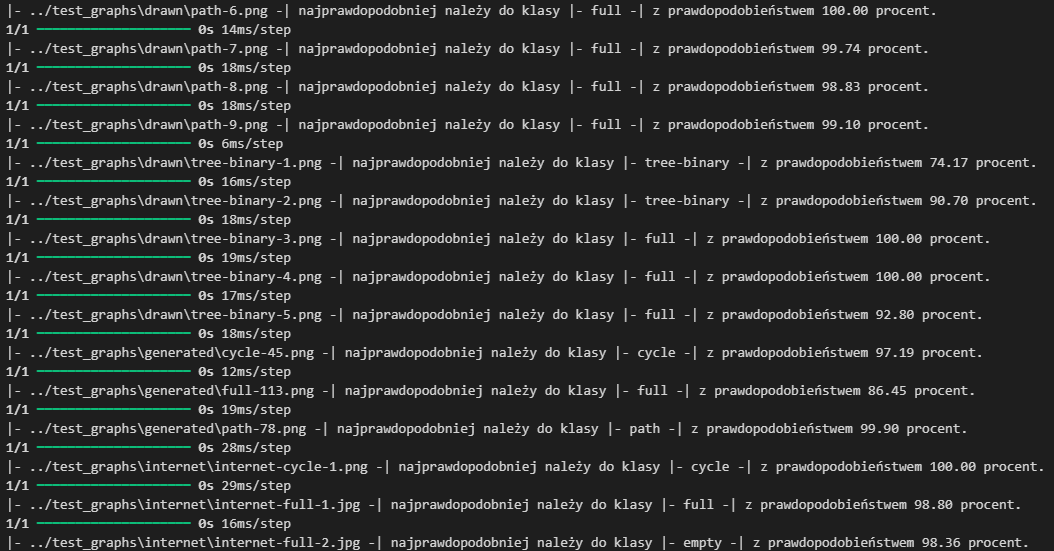
\includegraphics[height=7cm]{resources/tests/images/v3/base6_txt.png}
	\caption{Klasyfikacja obrazów zewnętrznych dla modelu podstawowego ze stałą krzywizną wierzechołków, liczba wierzchołków = 6}
	\label{Fig:tests-base-2}
\end{figure}
\FloatBarrier

\begin{figure}[ht]
	\centering
	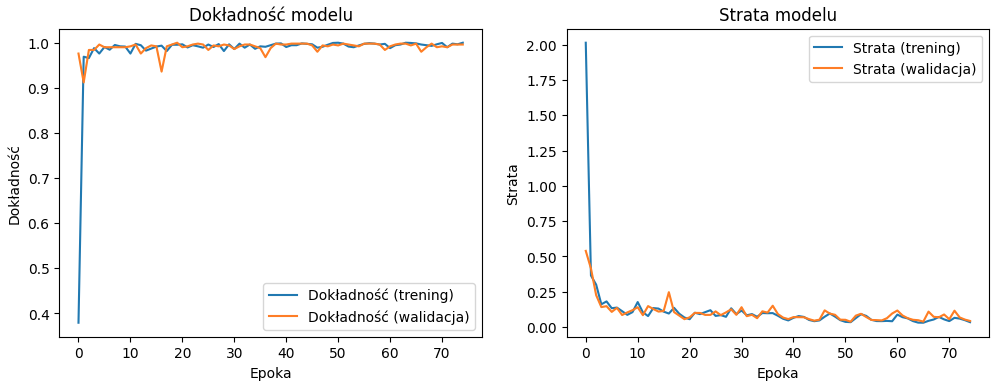
\includegraphics[height=5.5cm]{resources/tests/images/v3/base7_img.png}
	\caption{Wyniki testów dla modelu podstawowego z losową krzywizną wierzechołków, liczba wierzchołków = 7}
	\label{Fig:tests-base-1}
\end{figure}
\FloatBarrier

\begin{figure}[ht]
	\centering
	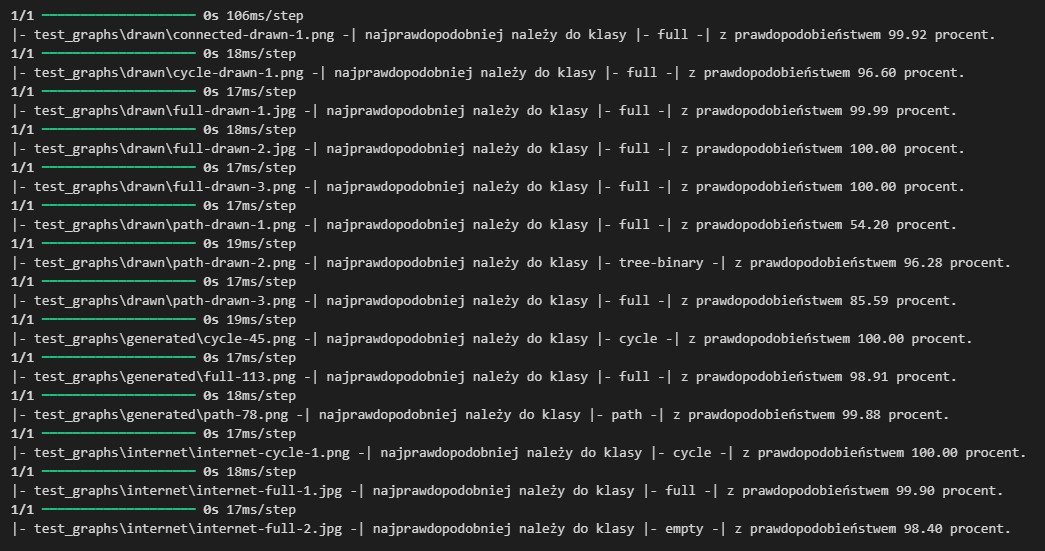
\includegraphics[height=7cm]{resources/tests/images/v3/base7_txt.png}
	\caption{Klasyfikacja obrazów zewnętrznych dla modelu podstawowego z losową krzywizną wierzechołków, liczba wierzchołków = 7}
	\label{Fig:tests-base-2}
\end{figure}
\FloatBarrier